\documentclass{article}

% if you need to pass options to natbib, use, e.g.:
%     \PassOptionsToPackage{numbers, compress}{natbib}
% before loading neurips_2020

% ready for submission
% \usepackage{neurips_2020}

% to compile a preprint version, e.g., for submission to arXiv, add add the
% [preprint] option:
%     \usepackage[preprint]{neurips_2020}

% to compile a camera-ready version, add the [final] option, e.g.:
%     \usepackage[final]{neurips_2020}

% to avoid loading the natbib package, add option nonatbib:
\usepackage[nonatbib]{neurips_2020}
\usepackage[utf8]{inputenc} % allow utf-8 input
\usepackage[T1]{fontenc}    % use 8-bit T1 fonts
\usepackage{hyperref}       % hyperlinks
\usepackage{url}            % simple URL typesetting
\usepackage{booktabs}       % professional-quality tables
\usepackage{amsfonts}       % blackboard math symbols
\usepackage{nicefrac}       % compact symbols for 1/2, etc.
\usepackage{microtype}      % microtypography
\usepackage{mathtools}
\usepackage{amsmath}
\usepackage{makecell}
\usepackage{bbm}
\usepackage{graphicx}

\DeclareMathOperator*{\argmax}{arg\,max}
\DeclareMathOperator*{\argmin}{arg\,min}

\title{Do (wo)men talk too much in films?}

% The \author macro works with any number of authors. There are two commands
% used to separate the names and addresses of multiple authors: \And and \AND.
%
% Using \And between authors leaves it to LaTeX to determine where to break the
% lines. Using \AND forces a line break at that point. So, if LaTeX puts 3 of 4
% authors names on the first line, and the last on the second line, try using
% \AND instead of \And before the third author name.

\author{%
  Johannes Graner \\
  % examples of more authors
  \And
  Isak Dahlqvist \\
  % Affiliation \\
  % Address \\
  % \texttt{email} \\
  \AND
  William Norman \\
  % Affiliation \\
  % Address \\
  % \texttt{email} \\
  % \And
  % Coauthor \\
  % Affiliation \\
  % Address \\
  % \texttt{email} \\
  % \And
  % Coauthor \\
  % Affiliation \\
  % Address \\
  % \texttt{email} \\
}

\begin{document}

\maketitle

\begin{abstract}
  
\end{abstract}

\newpage

\section{Introduction}

\section{Methods}
We have chosen to focus on approaches using logistic regression, k-NN, LDA and QDA to classify the lead actor's gender.

In order to make the methods as comparable as possible, we have used a common set of transformations of the input variables for all tested methods.

\subsection{Input transformations}
In the given dataset, there are columns for the total number of words spoken as well as the number of words spoken by the lead, the co-lead etc. This could present a problem since if we compare a movie where the lead says 10 out of 100 total words and another movie where the lead says 100 out of 1000 words, most models would think that the lead speaks more in the second movie and miss the fact that the \textit{proportion} of words spoken by the lead is the same. For that reason we have transformed several input variables to express a proportion instead of absolute numbers. We also believe it might be important to have a dummy variable indicating if the lead or the co-lead is oldest. All transformations are given in Table \ref{tab:transformations}.

\begin{table}[h!]
	\centering
	\begin{tabular}{ccc}
		Original column & New column & Transformation \\
		\midrule
		Number of words lead & \makecell{Proportion of \\ words lead} & $\frac{\text{Number of words lead}}{\text{Total words}}$ \\
		N/A & \makecell{Proportion of \\ words co-lead} & $\frac{\text{Number of words lead - Difference in words lead and co-lead}}{\text{Total words}}$ \\
		\makecell{Difference in words \\ lead and co-lead} & \makecell{Ratio words \\ co-lead lead} & $\frac{\text{Proportion of words co-lead}}{\text{Proportion of words lead}}$ \\
		Number words female & \makecell{Proportion of \\ words female} & $\frac{\text{Number words female}}{\text{Total words - Number of words lead}}$ \\
		\makecell{Number of \\ female actors} & \makecell{Proportion of \\ female actors} & $\frac{\text{Number of female actors}}{\text{Number of female actors + Number of male actos}}$ \\
		\makecell{Number of \\ male actors} & \makecell{Number of actors} & \makecell{Number of male actors + \\ Number of female actors} \\
		N/A & Older lead & $\begin{cases} 1, \text{Age lead > Age Co-Lead} \\ 0, \text{else} \end{cases}$
	\end{tabular}
	\label{tab:transformations}
	\caption{Transformations of input variables.}
\end{table}

Note that when determining 'Proportion of words female', this should only measure the words spoken by non-lead female actors so we have to subtract the lead's contribution to the total number of words.

The column 'Number of male actors' was dropped since all necessary information in this column is contained in 'Proportion of female actors' together with 'Number of actors'.

In order to improve regularization and k-NN, all remaining numerical input variables where centered and scaled by their standard deviation. This means that columns with proportions have values in the unit interval $[0,1]$ and the other numerical variables have values that are of roughly the same magnitude.

\subsection{Logistic Regression}
Logistic regression is a \textit{general linear model} (GLM), i.e. the relationship between the data $X \in \mathcal{X} \subseteq \mathbb{R}^p$ and the outcome $Y$ is on the form
\begin{equation}
	E(Y|X) = g^{-1}(X \cdot \beta)
\end{equation}
where $\beta \in \mathbb{R}^p$ and $g$ is the link function. In the case of logistic regression, $Y|X \sim Ber(p)$ and the canonical link function is the logit link $g(x) = \log \left( \frac{x}{1 - x} \right)$ with $g^{-1}(x) = \frac{\exp(x)}{1 + \exp(x)}$. Since $Y|X \sim Ber(p)$, we get $E(Y|X) = p = g^{-1}(X \cdot \beta)$. In other words, $P(Y = 1 | X = x) = g^{-1}(x \cdot \beta)$, which we can use to predict $Y$ given data $x$.

To do the regression, we find $\hat \beta \in \argmin_\beta \sum_{i=1}^{n} (y_i - \hat y(x_i; \beta))^2$ where $\hat y(x;\beta) = g^{-1} (x \cdot \beta)$. This minimizes the mean squared error (MSE) loss function. A potential problem with this approach is that there are no restrictions on the components of $\beta$ and that can lead to overfitting, especially if $n$ is not much larger than $p$. To address that issue, one can introduce regularization.

In general, regularization is done by adding a penalizing term to the loss function that restricts $\beta$ in some way. If $L(\beta; x_i,y_i)$ is the loss function before regularization, we instead consider the new loss function $L(\beta; x_i,y_i) + \lambda R(\beta)$ and find $\hat \beta_{reg} \in \argmin_\beta \left( L(\beta; x_i, y_i) + \lambda R(\beta) \right)$. $R$ is some penalizing function and $\lambda$ is a hyper-parameter that can be tuned. The two most common forms of regularization is LASSO and Ridge regression.

LASSO regression uses $L_1$-regularization, meaning that $R_{LASSO}(\beta) = ||\beta||_1 =  \sum_{i=1}^{p} |\beta_i|$ while Ridge regression uses $L_2$-regularization, $R_{Ridge}(\beta) = ||\beta||_2^2 = \sum_{i=1}^{p} \beta_i^2$.

In order to find a value of $\lambda$ that performs well on the data, cross-validation is used to find the optimal value in a finite set $\Lambda = \{ \lambda_1,\dots,\lambda_k \}$. Cross-validation works by splitting the data into $n$ equally sized partitions and training the data separately on the $n$ choices of $n-1$ partitions and testing on the partition that was left out. The test error $E_{new}$ is estimated by the mean misclassification rate across the partitions. This procedure is repeated for each $\lambda_j \in \Lambda$ and the value resulting in the lowest estimated test error is chosen.

Since cross-validation is used to estimate the hyper-parameter $\lambda$, this method cannot be used to estimate the test error of the whole procedure. Instead, the dataset has to be split into a training set and a testing set with a specified fraction of the total data in each set. The whole procedure above is done on the training set and the test error is estimated by evaluating the performance of the model on the testing set. However, this can yield significantly different estimates of the test error since only one split into training and testing data is considered. To get a better estimate of the actual testing error, a bootstrap procedure is performed.

Since the full dataset is an iid sample from some unknown distribution, the estimated test error $\hat E_{new}$ is a random variable. By repeating the whole procedure $B$ times (i.e. $B$ independent splits into training and testing data and subsequent fitting and cross-validation), a bootstrap sample of $\hat E_{new}$ is obtained which can be used to estimate the distribution (or at least properties thereof) of $\hat E_{new}$. This is very computationally intensive but gives a much clearer view of the variability of the test error compared to just computing it for one split.

\subsection{k-Nearest Neighbors}
The $k$-nearest neighbors ($k$-NN) method is based on the simple principle of finding the $k$ closest neighboring points with respect to the input data $X \in \mathcal{X} \subseteq \mathbb{R}^p$. In the case of Classification the outcome $Y$ is then determined by a majority vote among the $k$ nearest data points. The method is closely related to the idea that if a test data point is close to some training data point then the prediction should be that they have the same outcome $Y$.

The algorithm for k-NN can be implemented in a simple manner with a brute force algorithm measuring the distance from the test data point $\boldsymbol{x_{\star}}$ to each training data point $\boldsymbol{x_{i}}$, where $i = 1,...,n$ using some distance function $d(x,y)$. It is normal to use the Minkowski distance of order $p$ which is given by

\begin{equation}
	d(\boldsymbol{x},\boldsymbol{y}) = \left( \sum_{i=1}^{n} |x_{i} - y_{i}|^{p} \right)^{\frac{1}{p}}\textit{, where } \boldsymbol{x} = (x_1,...,x_p),\boldsymbol{y}=(y_1,...,y_p)
	\in \mathbb{R}^p.
\end{equation}

Where $p=1$ is the Manhattan distance, and when $p=2$ we have the Euclidean distance of course any distance function could be used.
The brute force algorithm for $k$-NN is given by 
\par\noindent\rule{\textwidth}{0.4pt}
\begin{enumerate}
 \item Calculate the distance $d(\boldsymbol{x_{i}},\boldsymbol{x_{\star}})$ for each $i = 1,...,n$
 \item Set $\mathcal{N}_{\star} = \{ \boldsymbol{x_i}: \textit{Where } \boldsymbol{x_i} \textit{ is one of the k nearest points} \}$
 \item Return $\hat{y}(\boldsymbol{x_{\star}}) = \text{MajorityVote}\{y_j : j \in \mathcal{N}_{\star}\} $
\end{enumerate}
\par\noindent\rule{\textwidth}{0.4pt}

\ref{kursbok}A problem with the brute force algorithm is that all the training data has to be stored and each distance has to be calculated which can be rather computer intensive. There are however algorithms as the ball-tree and k-d tree which speeds up these calculations. The general principle is still the same, exactly how these algorithms are performed are thus left out of the report.

In this case we let the Minkowski distance be our distance function and we let $p$ and $k$ be hyper-parameters which are to be tuned. This is done in an analogous manner as in the case of finding the hyper-parameter $\lambda$ in the Logistic regression case above. 

Weighted $k$-NN is an alternative approach to the normal $k$-NN where the $k$ nearest neigbors also are weighted based on how far or close from the test data point they actually are effecting the majority vote such that for example closer points have "stronger" vote. In our case we tested between \textit{uniform} weights (Standard $k$-NN) and \textit{distance} weights where the weight points equals

\begin{equation}
    \dfrac{1}{d(\boldsymbol{x_{\star}, \boldsymbol{x_i}})}, 
\end{equation}
for each of the k-nearest neighbors, this results in giving closer neighbors a stronger influence.
\ref{https://scikit-learn.org/stable/modules/generated/sklearn.neighbors.KNeighborsClassifier.html}

\subsection{LDA and QDA}
For classification we construct a discriminative classifier from a generative model based on Bayes' theorem for the classes $m=1,2,..,M$
\begin{equation}
    p(y=m \mid \boldsymbol{x}) = \frac{ p(\boldsymbol{x} \mid y=m) p(y=m)}
    {\sum_{i=1}^{M} p(\boldsymbol{x} \mid y=i)p(y=i)}.
\end{equation}
We estimate the \textit{uninformative prior probability} as $\hat{p}(y=m) = \frac{n_m}{n}$ where $n_m = \sum_{i=1}^{n} \mathbbm{1}\{y_i=m\}$ and assume that $p(\boldsymbol{x} \mid y=m)$ is a normal density with expected value $\mu_m$ and covariance matrix $\Sigma_m$. The assumption that distinguishes LDA and QDA is that for LDA we assumes that $\Sigma_1=\Sigma_2=...=\Sigma_M$ but for QDA we make no such assumption, that is, we allow for the covariance matrices to differ. A consequence is that LDA is a special case of QDA, hence QDA is a model of higher complexity. The estimates for the normal distribution parameters for each class is given by
\begin{align}
    \hat{\mu}_m &= \frac{1}{n_m} \sum_{i:y_i=m} \boldsymbol{x_i}, \\
    \hat{\Sigma}_m &= \frac{1}{n_m-1}\sum_{i:y_i=m} (\boldsymbol{x}_i-\hat{\mu}_m)(\boldsymbol{x}_i-\hat{\mu}_m)^T.
\end{align}
The \textit{pooled covariance estimate} (weighted average of the covariance matrix estimates within each class) is given by
\begin{equation}
    \hat{\Sigma} = \frac{\sum_{m=1}^{M} (n_m-1)\hat{\Sigma}_m}{\sum_{m=1}^{M} (n_m-1)}=\frac{1}{n-M}\sum_{m=1}^{M}\sum_{i:y_i=m} (\boldsymbol{x}_i-\hat{\mu}_m)(\boldsymbol{x}_i-\hat{\mu}_m)^T.
\end{equation}
Finally we may express the discriminant analysis classifier as
\begin{equation}
    \hat{p}(y=m \mid \boldsymbol{x}) = \frac{n_m\mathcal{N}(\boldsymbol{x} \mid \hat{\mu}_m, \hat{\Sigma})}{\sum_{i=1}^{M} n_i\mathcal{N}(\boldsymbol{x} \mid \hat{\mu}_m, \hat{\Sigma})}
\end{equation}
where $\mathcal{N}(\boldsymbol{x} \mid \mu,\Sigma)=\frac{1}{(2\pi)^{M/2}\mid\Sigma\mid^{1/2}}\exp{[-\frac{1}{2}(\boldsymbol{x}-\mu_m)^T\Sigma_m^{-1}(\boldsymbol{x}-\mu_m)]}$ is the density function for the normal distribution with mean $\mu$ and covariance matrix $\Sigma$.

\section{Results}

\subsection{Logistic Regression}

When comparing different models, it is important to have a baseline, or a null model to compare against. In this case, an obvious null model is the constant model that always predicts the same outcome regardless of input. The best null model is the one with highest accuracy, i.e. the constant model that predicts the most frequently occurring outcome. The model that always predicts a male lead has an accuracy of 0.756 and is thus chosen as the baseline.

For all logistic regression models fitted, the set of regularization parameters, $\Lambda$, consisted of 10 logarithmically spaced values between $10^{-4}$ and $10^4$. This was the default value in the methods from scikit learn and having more densely packed values did not affect the model performance in any appreciable way. The number of folds used in cross-validation was also 10, no improvement was observed by increasing this value.

The model performance was measured by accuracy (1 - misclassification rate) and AUC (area under ROC curve). In Tables \ref{tab:logreg_table_70} and \ref{tab:logreg_table_90}, the accuracy and AUC are estimated using the mean of 100 bootstrap samples in the case of LASSO regression and 400 in the case of Ridge regression. The reason for having different sample sizes is that computing the LASSO regression is much more computationally demanding.

\begin{table}[h!]
	\centering
	\begin{tabular}{cccc}
		Input & Regularization & Accuracy & AUC \\
		\midrule
		Before transformations & None & 0.870 & 0.878 \\
		& LASSO & 0.871 & 0.880 \\
		& Ridge & 0.871 & 0.880 \\
		\midrule
		After transformations & None & 0.893 & 0.920 \\
		& LASSO & 0.895 & 0.921 \\
		& Ridge & 0.894 & 0.921 \\
	\end{tabular}
	\caption{Accuracy and AUC for logistic regression models. 70\% training data.}
	\label{tab:logreg_table_70}
\end{table}

\begin{table}[h!]
	\centering
	\begin{tabular}{cccc}
		Input & Regularization & Accuracy & AUC \\
		\midrule
		Before transformations & None & 0.876 & 0.878 \\
		& LASSO & 0.875 & 0.883 \\
		& Ridge & 0.871 & 0.880 \\
		\midrule
		After transformations & None & 0.895 & 0.924 \\
		& LASSO & 0.897 & 0.924 \\
		& Ridge & 0.898 & 0.923 \\
	\end{tabular}
	\caption{Accuracy and AUC for logistic regression models. 90\% training data.}
	\label{tab:logreg_table_90}
\end{table}

We see that the regularization does not affect the model performance much. LASSO and Ridge regularization perform almost identically and yield at best around 0.3\% extra accuracy but considering that the different splits of the data yielded estimated test errors in a range from 0.8 to 0.98, we cannot reject that regularization does not matter in this case.


\subsubsection{k-Nearest Neighbors}

When hyper-tuning the algorithm the set of $p$-values and $k$-values were given by $\{1,1.25,1.5,...,4\}$ and $\{1,2,3,...,25\}$ respectively. The number of folds used in cross-validation was again set to 10. It was found that $p = 2$ (Euclidean distance) and $k = 4$ performed best for our data set. Using these parameters the k-NN algorithm was tested and performance was measured with the mean of 100 bootstraps samples as before, the size of the sample was chosen with regards to k-NN being computationally demanding. The results are summarized in Table \ref{tab:k_nn_table_10} and Table \ref{tab:k_nn_table_20} below.
 

\begin{table}[!h]
\centering
\begin{tabular}{cccc}
		Input & Weighted k-NN & Accuracy & AUC \\
		\midrule
		Before transformations & Uniform & 0.745 & 0.675 \\
	    & Distance & 0.780 & 0.688 \\
		\midrule
		After transformations & Uniform & 0.864 & 0.883 \\
		& Distance & 0.872 & 0.888 \\
	\end{tabular}
	\caption{Accuracy and AUC for k-NN models. 70\% training data.}
	\label{tab:k_nn_table_10}
\end{table}


\begin{table}[!h]
\centering
\begin{tabular}{cccc}
        Input & Weighted k-NN & Accuracy & AUC \\
		\midrule
		Before transformations & Uniform & 0.750 & 0.678 \\
	    & Distance & 0.783 & 0.693 \\
		\midrule
		After transformations & Uniform & 0.875 & 0.891 \\
		& Distance & 0.882 & 0.901 \\
	\end{tabular}
	\caption{Accuracy and AUC for k-NN models. 90\% training data.}
	\label{tab:k_nn_table_20}
\end{table}

It is obvious that k-NN is drastically improved by transforming the data, before transformations the model performance was even outperformed or just slightly better than the best null model. Weighted k-NN with the \textit{distance} weight seemed to perform better than the \textit{uniform} weight both before and after the transformation, the impact seems to be $0.7-0.8\%$ extra accuracy after transformation and almost $3\%$ extra accuracy before transformations. 

\subsection{LDA and QDA}
The given dataset was bootstrapped 400 times and both DA models were tested before and after input transformations.
\begin{table}[h!]
	\centering
	\begin{tabular}{cccc}
		Input & DA Model & Mean Accuracy & Mean AUC \\
		\midrule
		Before transformations
		& LDA & 0.856 & 0.870 \\
	    & QDA & 0.818 & 0.849 \\
		\midrule
		After transformations
		& LDA & 0.893 & 0.913 \\
		& QDA & 0.933 & 0.966 \\
	\end{tabular}
	\caption{Mean Accuracy and Mean AUC for discriminant analysis models. 70\% training data.}
	\label{tab:discanal_table_70}
\end{table}
\begin{table}[h!]
	\centering
	\begin{tabular}{cccc}
		Input & DA Model & Mean Accuracy & Mean AUC \\
		\midrule
		Before transformations
		& LDA & 0.866 & 0.877 \\
	    & QDA & 0.840 & 0.869 \\
		\midrule
		After transformations
		& LDA & 0.903 & 0.915 \\
		& QDA & 0.942 & 0.977 \\
	\end{tabular}
	\caption{Mean Accuracy and Mean AUC for discriminant analysis models. 90\% training data.}
	\label{tab:discanal_table_90}
\end{table}
From the results it is clear that QDA seems to have better performance after transformations. It is unclear which method performs better before the transformation because for QDA the variance is high. The high variance can for QDA can be explained by the fact that the original inputs are close to being colinear making $\Sigma$ close to being singular which in turn results in an inaccurate matrix inversion. For example, the standard deviation of accuracy and AUC of the QDA classifier, before transformations, on 400 bootstrapped datasets with 90\% training data were 0.076 and 0.081 respectively compared to 0.021 and 0.019 after transformations ceteris paribus.

--Based on the results it seems that LDA is not complex enough of a model for this task. SKRIV OM VARFÖR QDA ÄR BÄTTRE ÄN LDA FÖR DET HÄR
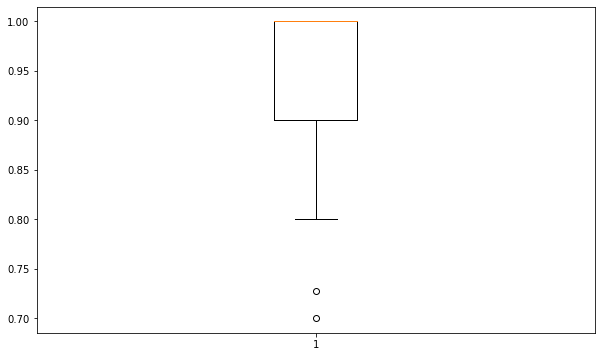
\includegraphics[scale=0.3]{boxplotQDA.png}
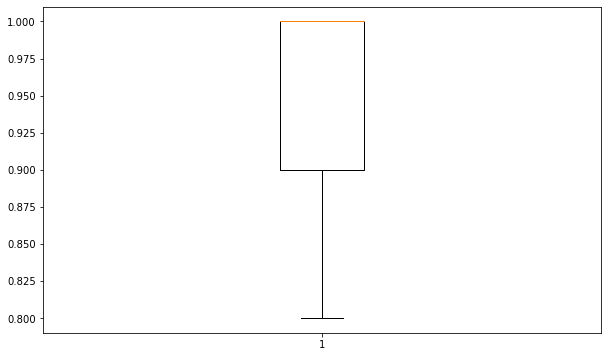
\includegraphics[scale=0.3]{boxplotQDA90.png}
-- några fall av väldigt dåliga resultat (70-75\%) går detta att undvika? har johannes modell lika? är det pga otur i uppdelningen av datan vid cross validation??
-- 0.9428 accuracy cross validation 100 folds 70\% training data
-- ENDAST EFTER TRANSFORMATION
-- 0.9420 accuracy cross validation 100 folds 90\% training data

\section{Conclusions}
It seems like $k$-NN was the worst performing of the models worth noting is the drastic effect that data transformations has on the $k$-NN model, performing at the same level as the baseline model before any transformations. Since the model is somewhat "blind" to feature importance and is greatly affected by variances in the data. Normalization of the data is thus crucial for good results.



\section{Feature Importance}

\end{document}
